\documentclass[11pt,a4paper]{article}
\usepackage[T1]{fontenc}
\usepackage[utf8]{inputenc}
\usepackage[spanish,es-nodecimaldot]{babel}
\usepackage{amsmath,amssymb,bm,booktabs,array,graphicx,geometry,xcolor,hyperref}
\geometry{margin=2.15cm}
\hypersetup{colorlinks=true,linkcolor=blue,urlcolor=blue,citecolor=blue}
\setlength{\parskip}{5pt}
\setlength{\parindent}{0pt}

\newcommand{\E}{\ensuremath{\bm E}}
\newcommand{\F}{\ensuremath{\bm F}}
\newcommand{\Svec}{\ensuremath{\bm S}}
\newcommand{\evec}{\ensuremath{\bm e}}
\newcommand{\Dfour}{\ensuremath{D_4}}
\newcommand{\W}{\ensuremath{W}}
\newcommand{\FOM}{\textsc{FOM}}
\newcommand{\HPROM}{\textsc{HPROM--ANN}}
\newcommand{\PANN}{\textsc{PANN--}\Dfour}
\newcommand{\ICNN}{\textsc{ICNN--}\Dfour}
\newcommand{\PConvPANN}{\textsc{PConv--PANN--}\Dfour}
\newcommand{\ICKAN}{\textsc{ICKAN--}\Dfour}
\newcommand{\PConvICKAN}{\textsc{PConv--ICKAN--}\Dfour}
\newcommand{\keybox}[1]{\begin{center}\fcolorbox{blue!55!black}{blue!4}{\parbox{0.91\linewidth}{#1}}\end{center}}
\newcommand{\warnbox}[1]{\begin{center}\fcolorbox{red!65!black}{red!4}{\parbox{0.91\linewidth}{#1}}\end{center}}

\title{Modelo \PANN{} para la respuesta constitutiva homogenizada\\
de un RVE hiperelástico con simetría cuadrada\\[3pt]
\large Memoria técnica: formulación, entrenamiento, verificación y resultados}
\author{Borrador metodológico para discusión científica}
\date{27 de julio de 2026}

\begin{document}
\maketitle

\begin{abstract}
Este documento formula y documenta una red neuronal informada por la física
para aproximar la energía homogenizada de un RVE hiperelástico bidimensional.
El modelo recibe la deformación macroscópica de Green--Lagrange, produce una
única energía escalar y obtiene la tensión por derivación automática. La
arquitectura incorpora de forma exacta la objetividad, el estado de referencia,
la consistencia energía--tensión y la simetría efectiva cuadrada \(\Dfour\) del
RVE. Se describen el conjunto de datos, la función de pérdida, la selección de
arquitectura y el protocolo final de entrenamiento con diez trayectorias
Stage--1 y evaluación ciega en Stage--10. El modelo final alcanza errores
relativos \(L^2\) de \(0.0522\%\) en energía y \(0.1689\%\) en tensión global
en Stage--10. También se delimitan explícitamente las propiedades que esta
arquitectura \emph{no} garantiza: convexidad, policonvexidad y estabilidad
global frente al colapso de volumen.
Como extensión separada y deliberadamente más restrictiva, se construye una
energía \PConvPANN{} que es policonvexa por diseño y posee barrera frente a
\(J=\det\F\to0^+\) y crecimiento cuando \(J\to\infty\). Esta segunda
arquitectura permite distinguir con datos qué se gana en garantías y qué se
pierde en fidelidad.
Finalmente se reentrenan dos ICKAN desde cero bajo el mismo protocolo: una
ICKAN directa como control flexible y una \PConvICKAN{} que usa menores
direccionales, es policonvexa por construcción y mejora de forma marcada la
primera extensión policonvexa, aunque no alcanza la precisión de la PANN
libre.
\end{abstract}

\textbf{Palabras clave:} homogeneización computacional; hiperelasticidad
finita; RVE; redes neuronales informadas por la física; energía constitutiva;
simetría material cuadrada.

\newpage

\section{Objetivo y alcance}

El problema de partida es un RVE hiperelástico no lineal resuelto mediante un
modelo de elementos finitos de alta fidelidad (\FOM). Para cada estado de
deformación macroscópica, dicho modelo microscópico proporciona una energía
homogenizada y una tensión macroscópica. Su coste hace conveniente sustituirlo,
en la escala macro, por un modelo constitutivo reducido.

El objetivo concreto no es ajustar tres curvas de tensión independientes. Se
busca aprender una función de energía macroscópica
\[
  \W_\theta^M(\E),
\]
de modo que la tensión se deduzca de la misma superficie energética. Esta
decisión impone una relación constitutiva integrable entre energía y tensión y
evita que ambas salidas sean incompatibles entre sí.

El alcance del trabajo es el RVE y la familia de trayectorias disponible. La
red no pretende sustituir el \FOM{} fuera del dominio de deformación entrenado
ni demostrar, por sí sola, estabilidad material global. Estas distinciones son
importantes para interpretar correctamente tanto las garantías como los
resultados numéricos.

\section{Magnitudes constitutivas y objetividad}

\subsection{Entrada macroscópica}

La entrada física es la deformación de Green--Lagrange
\[
 \E=\frac12(\F^T\F-\bm I)
 =\begin{bmatrix}
 E_{xx} & \gamma_{xy}/2\\
 \gamma_{xy}/2 & E_{yy}
 \end{bmatrix},
 \qquad
 \evec=[E_{xx},E_{yy},\gamma_{xy}]^T,
 \qquad
 \gamma_{xy}=2E_{xy}.
\]
Por tanto, \(E_{xx}\) y \(E_{yy}\) son deformaciones normales en las
direcciones horizontal y vertical, respectivamente, y \(\gamma_{xy}\) es la
deformación cortante ingenieril. En los archivos originales estas mismas
componentes se denominan \(E_{11}\), \(E_{22}\) y \(\gamma_{12}\).

\subsection{Por qué esta elección impone objetividad}

La objetividad exige que un cambio de observador mediante una rotación rígida
\(\bm Q\), con \(\bm Q^T\bm Q=\bm I\), no modifique la energía material:
\[
 \W^M(\bm Q\F)=\W^M(\F).
\]
Al usar \(\E\) como entrada, la propiedad se cumple antes de entrenar la red:
\[
 \E(\bm Q\F)
 =\frac12\left((\bm Q\F)^T\bm Q\F-\bm I\right)
 =\frac12\left(\F^T\F-\bm I\right)
 =\E(\F).
\]
En consecuencia, cualquier función \(\W_\theta^M(\E)\) cumple objetividad con
respecto a superposiciones de rotación rígida. Esta afirmación no significa que
el material sea isótropo; la isotropía se refiere a una rotación de la
\emph{estructura material}, no a un cambio de observador.

\subsection{Energía y tensión conjugada}

El \FOM{} entrega una energía volumétrica macroscópica \(\W^M\) y la tensión
conjugada de segundo Piola--Kirchhoff
\[
 \Svec^M=[S_{xx}^M,S_{yy}^M,S_{xy}^M]^T.
\]
Con la convención de cizalla anterior, la identidad de trabajo es
\[
 d\W^M
 =S_{xx}^M\,dE_{xx}
 +S_{yy}^M\,dE_{yy}
 +S_{xy}^M\,d\gamma_{xy}.
 \label{eq:work}
\]
La red se formula para satisfacer esa misma conjugación:
\[
 \boxed{\qquad
 \Svec_\theta(\evec)
 =\frac{\partial\W_\theta^M}{\partial\evec}.
 \qquad}
 \label{eq:stress-gradient}
\]
Así, la tensión no es una segunda salida ajustada con parámetros distintos:
es la pendiente de la energía que se ha aprendido.

La literatura de policonvexidad suele escribir la misma energía como
\(\Psi(\F)\) y emplear el primer Piola--Kirchhoff
\(\bm P=\partial\Psi/\partial\F\). No hay contradicción con nuestra medida:
\[
 \bm P=\F\Svec,
 \qquad \Svec=\F^{-1}\bm P,
 \qquad
 \bm\sigma=J^{-1}\F\Svec\F^T.
 \label{eq:stress_measures}
\]
Por tanto, un modelo de energía puede compararse con HPROM--ANN en segundo
Piola, como se hace aquí, y convertir ambos a primer Piola con el mismo
\(\F\) macroscópico si esa representación resulta necesaria. No requiere
reentrenar ninguna de las dos redes.

\section{Simetría material efectiva: cuadrada, no isótropa}

\subsection{Significado de \texorpdfstring{\(\Dfour\)}{D4}}

La celda, su microestructura y las condiciones empleadas en el problema son
invariantes bajo las simetrías de un cuadrado. El grupo correspondiente,
\(\Dfour\), contiene las rotaciones de \(0^\circ\), \(90^\circ\),
\(180^\circ\) y \(270^\circ\), así como cuatro reflexiones. Para un tensor
simétrico de segundo orden, las ocho matrices generan sólo cuatro
transformaciones distintas de \((E_{xx},E_{yy},\gamma_{xy})\):
\[
\begin{array}{c|c}
\text{acción material} & (E_{xx},E_{yy},\gamma_{xy})\ \text{transformado}\\
\toprule
\text{identidad} & (E_{xx},E_{yy},\gamma_{xy})\\
\text{rotación de }90^\circ & (E_{yy},E_{xx},-\gamma_{xy})\\
\text{reflexión respecto a un eje} & (E_{xx},E_{yy},-\gamma_{xy})\\
\text{reflexión respecto a una diagonal} & (E_{yy},E_{xx},\gamma_{xy})
\end{array}
\label{tab:d4actions}
\]

El principio general es el de \emph{simetría material}: una transformación
pertenece al grupo de simetría si deja invariante la respuesta constitutiva
\cite{gurtin2010}. En la nomenclatura de grupos puntuales
cristalográficos, la simetría cuadrada con reflexiones se escribe
habitualmente \(4mm\), o \(C_{4v}\) en notación de Schoenflies; su acción en
el plano es isomorfa al grupo diédrico \(\Dfour\) \cite{nye1985}. En esta
memoria se usa \(\Dfour\) porque describe directamente las rotaciones y
reflexiones que se aplican al tensor bidimensional.

La simetría material esperada se expresa como
\[
 \W^M(\bm R^T\E\bm R)=\W^M(\E),\qquad
 \Svec^M(\bm R^T\E\bm R)=\bm R^T\Svec^M(\E)\bm R,
 \qquad \bm R\in\Dfour.
 \label{eq:d4}
\]
La segunda igualdad se interpreta tensorialmente antes de volver a escribir
las tres componentes físicas de \(\Svec^M\).

\subsection{Por qué \texorpdfstring{\(\Dfour\)}{D4} no es isotropía}

Un material isótropo sería invariante para \emph{cualquier} ángulo de rotación.
La simetría \(\Dfour\) sólo autoriza el conjunto discreto de operaciones del
cuadrado. Una rotación material de \(45^\circ\), por ejemplo, no pertenece a
\(\Dfour\); por ello la respuesta no tiene por qué coincidir con la predicción
isótropa.

Esta diferencia no se asume sólo por motivos geométricos: se verificó
numéricamente con el \FOM. Para tres estados mixtos con cizalla, las
transformaciones de \(\Dfour\) dieron errores máximos relativos de
\(1.96\times10^{-6}\) en tensión y \(8.82\times10^{-7}\) en energía. En
cambio, al rotar materialmente \(45^\circ\), la discrepancia respecto a la
respuesta que predeciría isotropía fue entre \(0.28\%\) y \(1.56\%\) en
tensión, y entre \(0.105\%\) y \(0.371\%\) en energía. Al nivel de precisión
del \FOM, el RVE es por tanto compatible con \(\Dfour\), pero no con
isotropía completa.

\keybox{\textbf{Consecuencia para el modelo.} Imponer isotropía obligaría a
igualar respuestas que el \FOM{} distingue. No imponer ninguna simetría
obligaría a la red a reaprender relaciones conocidas. La restricción correcta
para este RVE es la simetría cuadrada \(\Dfour\).}

\section{Arquitectura \texorpdfstring{\PANN{}}{PANN-D4}}

\subsection{Red de energía base y promediado de grupo}

La red base \(w_\theta:\mathbb R^3\rightarrow\mathbb R\) es una MLP escalar
con tres capas ocultas de \(128\), \(128\) y \(64\) neuronas y activación
Softplus con parámetro \(\beta=4\). Esta red, por sí sola, no posee
necesariamente simetría cuadrada.

La energía cruda se transforma en una energía exactamente invariante mediante
el promedio de las cuatro acciones de la Tabla~\ref{tab:d4actions}:
\[
\begin{aligned}
\overline w_\theta(E_{xx},E_{yy},\gamma_{xy})=\frac14\big[&
w_\theta(E_{xx},E_{yy},\gamma_{xy})
{}+w_\theta(E_{yy},E_{xx},-\gamma_{xy})\\
&{}+w_\theta(E_{xx},E_{yy},-\gamma_{xy})
{}+w_\theta(E_{yy},E_{xx},\gamma_{xy})\big].
\end{aligned}
\label{eq:groupaverage}
\]
Como las cuatro entradas aparecen intercambiadas al aplicar cualquier
operación de \(\Dfour\), la media de la ecuación~\eqref{eq:groupaverage} no
cambia. La simetría no se aprende de forma aproximada: queda incorporada en
la arquitectura.

\subsection{Corrección del estado de referencia}

Una red neuronal genérica no garantiza ni energía ni tensión nulas en el
estado sin deformar. Para imponer ambas condiciones se define
\[
\boxed{
\W_\theta^M(\evec)
=\overline w_\theta(\evec)-\overline w_\theta(\bm0)
-\left.
\frac{\partial\overline w_\theta}{\partial\evec}
\right|_{\bm0}\cdot\evec .}
\label{eq:reference-correction}
\]
Al derivar esta expresión se obtiene la tensión de la
ecuación~\eqref{eq:stress-gradient}. De forma exacta, para cualquier conjunto
de pesos \(\theta\),
\[
 \W_\theta^M(\bm0)=0,\qquad
 \Svec_\theta(\bm0)=\bm0.
\]
La corrección no depende de disponer de una muestra de entrenamiento en el
origen; es una condición analítica de la arquitectura.

\subsection{Propiedades incorporadas y propiedades no demostradas}

\begin{center}
\small
\begin{tabular}{p{0.40\linewidth}ccp{0.29\linewidth}}
\toprule
Propiedad & \PANN{} & \ICNN{} & Razón\\
\midrule
Objetividad & sí & sí & La entrada es \(\E=\frac12(\F^T\F-\bm I)\).\\
Simetría material cuadrada & sí & sí & Promedio exacto sobre \(\Dfour\).\\
\(\W(\bm0)=0,\ \Svec(\bm0)=\bm0\) & sí & sí & Corrección de la ecuación~\eqref{eq:reference-correction}.\\
Consistencia energía--tensión & sí & sí & \(\Svec=\partial\W/\partial\evec\).\\
Convexidad en \(\E\) & no & sí & Sólo la ICNN restringe sus pesos.\\
Policonvexidad o estabilidad global en \(\F\) & no & no & No se usa una construcción policonvexa.\\
Barrera cuando \(\det\F\rightarrow0^+\) & no & no & No se introduce un término volumétrico singular.\\
\bottomrule
\end{tabular}
\end{center}

La ICNN fue analizada como alternativa con una garantía adicional de
convexidad en \(\E\). Sin embargo, convexidad en esta parametrización no
equivale a policonvexidad ni a convexidad de rango uno en \(\F\). De hecho, la
ICNN evaluada mostró curvatura de rango uno negativa de aproximadamente
\(-2.924\)~GPa en una prueba de compresión extrema y energía finita cuando el
volumen tiende a colapsar. Por ello no se atribuye a la ICNN una garantía de
estabilidad global que no posee.

\section{Datos, normalización y entrenamiento}

\subsection{Protocolo de datos}

Los datos de entrenamiento proceden de diez trayectorias \FOM{} denominadas
Stage--1. Contienen \(109\,460\) estados de deformación, energía y tensión
conjugada obtenida a partir de la energía microscópica. La trayectoria
Stage--10, compuesta por \(1\,151\) estados, queda completamente fuera de la
selección de modelo y del entrenamiento final.

La secuencia metodológica fue:
\[
\boxed{
\begin{array}{c}
\text{selección: Stage--1 trayectorias 1--8}\\
\downarrow\\
\text{validación interna: Stage--1 trayectorias 9--10}\\
\downarrow\\
\text{reentrenamiento final: las diez trayectorias Stage--1}\\
\downarrow\\
\text{una sola evaluación final: Stage--10}.
\end{array}}
\]
Así se evita elegir una arquitectura porque ajusta accidentalmente la
trayectoria que se usa para la comparación final con \HPROM.

\subsection{Normalización}

Se usa una escala escalar común de deformación y energía,
\[
 \bm x=\frac{\evec}{e_0},\qquad
 \widehat\W=\frac{\W}{W_0},\qquad
 \widehat{\Svec}=\frac{e_0}{W_0}\Svec.
\]
La relación física recuperada tras la derivación es
\[
 \Svec=\frac{W_0}{e_0}
 \frac{\partial\widehat\W}{\partial\bm x}.
\]
En el entrenamiento final se usaron \(e_0=2.0\) y
\(W_0=2.135640832\times10^9\)~Pa. Al ser la escala de deformación común a los
tres componentes, no altera las transformaciones de \(\Dfour\).

\subsection{Función de pérdida}

Para un lote de \(N\) muestras se definen las pérdidas normalizadas
\[
 \mathcal L_\W=
 \frac{\frac1N\sum_{i=1}^N(\widehat\W_i-\widehat\W_i^{\FOM})^2}
      {\frac1N\sum_{i=1}^N(\widehat\W_i^{\FOM})^2},
\]
\[
 \mathcal L_{\Svec,\mathrm{global}}=
 \frac{\frac1{3N}\sum_{i=1}^N\|\widehat{\Svec}_i-\widehat{\Svec}_i^{\FOM}\|_2^2}
      {\frac1{3N}\sum_{i=1}^N\|\widehat{\Svec}_i^{\FOM}\|_2^2},
\]
\[
 \mathcal L_{\Svec,\mathrm{componentes}}=
 \frac13\sum_{\alpha\in\{xx,yy,xy\}}
 \frac{\frac1N\sum_{i=1}^N
  (\widehat S_{\alpha,i}-\widehat S_{\alpha,i}^{\FOM})^2}
 {\frac1N\sum_{i=1}^N(\widehat S_{\alpha,i}^{\FOM})^2}.
\]
La función optimizada es
\[
\boxed{
\mathcal L=
0.65\,\mathcal L_\W+
1.00\left(
0.35\,\mathcal L_{\Svec,\mathrm{global}}+
0.65\,\mathcal L_{\Svec,\mathrm{componentes}}
\right).}
\label{eq:loss}
\]
El término global controla la respuesta de tensión como vector. El término por
componentes evita que \(S_{xy}\), de menor escala en gran parte de las
trayectorias, quede oculto por las tensiones normales.

El entrenamiento final usa AdamW, tasa de aprendizaje inicial
\(4\times10^{-4}\), \emph{weight decay} \(10^{-8}\), lotes de \(2\,048\)
muestras, recorte de gradiente de norma \(50\) y \(300\) épocas. La semilla
del modelo seleccionado es \(20260731\).

\section{Alternativas exploradas y selección}

La exploración se comunica mediante tres familias conceptualmente distintas,
no mediante una lista de hiperparámetros o semillas:

\begin{center}
\small
\begin{tabular}{p{0.26\linewidth}p{0.31\linewidth}p{0.31\linewidth}}
\toprule
Familia & Construcción & Resultado de la exploración\\
\midrule
\ICNN{} &
Energía con envolvente \(\Dfour\) y pesos restringidos para convexidad en
\(\E\). &
Añade convexidad en la entrada, pero presenta la peor fidelidad para este RVE.\\[2pt]
MLP con invariantes \(\Dfour\) &
La red recibe
\([E_{xx}+E_{yy},(E_{xx}-E_{yy})^2,\gamma_{xy}^2]\). &
La simetría se impone directamente, pero los términos cuadrados reducen la
sensibilidad de primer orden a la diferencia normal y a la cizalla cerca del
origen.\\[2pt]
\PANN{} final &
MLP directa en \([E_{xx},E_{yy},\gamma_{xy}]\), promedio de grupo y
corrección de referencia. &
Mantiene las garantías físicas necesarias y obtiene la mejor precisión.\\
\bottomrule
\end{tabular}
\end{center}

La Tabla~\ref{tab:selection} muestra los errores de selección en las
trayectorias internas 9--10, sin usar Stage--10.
\begin{table}[ht]
\centering
\caption{Selección de arquitectura con Stage--1: entrenamiento en
trayectorias 1--8 y validación en 9--10.}
\label{tab:selection}
\begin{tabular}{lcc}
\toprule
Modelo & error de energía & error de tensión global\\
\midrule
\ICNN{} & \(1.619\%\) & \(5.116\%\)\\
MLP con invariantes \(\Dfour\) & \(0.476\%\) & \(2.583\%\)\\
\PANN{} final & \(\mathbf{0.049\%}\) & \(\mathbf{0.296\%}\)\\
\bottomrule
\end{tabular}
\end{table}

\section{Extensión policonvexa con barrera volumétrica}

\subsection{Motivación y cambio de variable constitutivo}

La entrada \(\E\) no impide formular una energía policonvexa. Lo que no es
suficiente es imponer convexidad a una MLP genérica en \(\E\). La
policonvexidad es una propiedad de la energía escrita como función de \(\F\):
\[
 \Psi(\F)=G\bigl(\F,\operatorname{cof}\F,\det\F\bigr),
 \qquad G\ \text{convexa}.
 \label{eq:polyconvex_definition}
\]
No se puede recuperar un \(\F\) único a partir de \(\E\), ya que
\[
 \F=\bm R\bm U,\qquad
 \bm U=\sqrt{\bm I+2\E},
\]
con \(\bm R\) una rotación rígida arbitraria. Esto no es una pérdida de
información para una energía objetiva: se puede evaluar desde
\(\bm C=\bm I+2\E\). Sin embargo, la prueba de estabilidad debe hacerse
respecto a \(\F\) y sus menores, no respecto al Hessiano de una MLP en
\(\E\) \cite{ball1977,linka2023}.

Se construyó por ello una única extensión \PConvPANN{}, separada del
\PANN{} libre seleccionado. Su propósito no es reemplazar retrospectivamente
al surrogate preciso, sino comprobar de forma reproducible el coste de exigir
policonvexidad y crecimiento global para este RVE.

\subsection{Medidas objetivas con simetría \texorpdfstring{\(\Dfour\)}{D4}}

Sea \(\mathcal A\) un conjunto cerrado bajo las simetrías del cuadrado. En
la implementación contiene las direcciones axiales, las diagonales y las
órbitas completas de las direcciones de \(22.5^\circ\) y \(15^\circ\).
Para cada \(\bm a\in\mathcal A\) se definen
\[
 q^{F}_{\bm a}=\lVert\F\bm a\rVert^2
 =\bm a^T\bm C\bm a,
 \qquad
 q^{H}_{\bm a}=\lVert\operatorname{cof}\F\bm a\rVert^2
 =\bm a^T\operatorname{cof}(\bm C)\bm a,
 \qquad J=\sqrt{\det\bm C}.
 \label{eq:directional_minors}
\]
Por tanto, todas las cantidades se evalúan directamente desde la entrada
\(\E\). Los superíndices \(F\) y \(H\) identifican el menor utilizado; no
son dos salidas de tensión distintas.

El vector de características es
\[
 \bm q(\E)=
 \left[\{q^F_{\bm a}\}_{\bm a\in\mathcal A},
       \{q^H_{\bm a}\}_{\bm a\in\mathcal A},J,J^2\right]^T.
\]
Una ICNN \(h_\theta(\bm q)\) usa Softplus y pesos estrictamente positivos:
\[
 \bm z_1=\operatorname{Softplus}(\bm A_1\bm q+\bm b_1),
 \qquad
 \bm z_{\ell}=\operatorname{Softplus}
 (\bm A_\ell\bm q+\bm B_\ell\bm z_{\ell-1}+\bm b_\ell),
 \qquad
 h_\theta=\bm u^T\bm q+\bm v^T\bm z_L+b,
 \label{eq:monotone_icnn}
\]
con \(\bm A_\ell,\bm B_\ell,\bm u,\bm v>0\). En consecuencia,
\(h_\theta\) es convexa y no decreciente en cada componente de \(\bm q\).
La red usada tiene capas \((64,64,32)\). La simetría material se impone con
la misma media de grupo que en la ecuación~\eqref{eq:groupaverage}:
\[
 H_{\theta,\Dfour}(\evec)=
 \frac14\sum_{g\in\{1,R_{90},M_x,M_d\}}
 h_\theta\bigl(\bm q(g\evec)\bigr).
 \label{eq:pc_group_average}
\]

\subsection{Referencia, policonvexidad y crecimiento}

La corrección afín en \(\E\) de la ecuación~\eqref{eq:reference-correction}
no se puede reutilizar: en general destruiría la representación convexa en
los menores. En su lugar se define
\[
 \boxed{
 W_{\mathrm{pc}}(\E)=H_{\theta,\Dfour}(\E)-H_{\theta,\Dfour}(\bm0)
 -r\log J+\frac{\beta}{2}(J-1)^2,\qquad \beta>0.}
 \label{eq:pc_energy}
\]
El coeficiente se calcula, no se ajusta por separado,
\[
 r=\frac12\left[S^H_{xx}(\bm0)+S^H_{yy}(\bm0)\right]\ge0,
 \qquad \Svec^H=\frac{\partial H_{\theta,\Dfour}}{\partial\evec}.
 \label{eq:pc_reference_pressure}
\]
La simetría \(\Dfour\) implica \(\Svec^H(\bm0)=[r,r,0]^T\), mientras que
\[
 \left.\frac{\partial\log J}{\partial\evec}\right|_{\bm0}=[1,1,0]^T.
\]
Así, la arquitectura satisface exactamente
\[
 W_{\mathrm{pc}}(\bm0)=0,
 \qquad \frac{\partial W_{\mathrm{pc}}}{\partial\evec}(\bm0)=\bm0.
\]

La garantía central se ve escribiendo la misma energía como
\[
 W_{\mathrm{pc}}(\F)=G_\theta\bigl(\F,\operatorname{cof}\F,J\bigr).
\]
Cada \(q^F_{\bm a}\) es convexa en \(\F\), cada \(q^H_{\bm a}\) es
convexa en \(\operatorname{cof}\F\), y \(J\) y \(J^2\) son funciones
convexas de la variable independiente \(J>0\). Como \(h_\theta\) es
convexa y no decreciente componente a componente, la regla de composición
hace que \(G_\theta\) sea convexa en \((\F,\operatorname{cof}\F,J)\).
El promedio finito de la ecuación~\eqref{eq:pc_group_average}, el término
\(-r\log J\) y el término cuadrático preservan esa convexidad. Por tanto,
\[
 \boxed{W_{\mathrm{pc}}\ \text{es policonvexa en el sentido de
la ecuación~\eqref{eq:polyconvex_definition}.}}
\]
Además,
\[
 \lim_{J\to0^+}W_{\mathrm{pc}}=+\infty
 \quad\text{por }-r\log J,
 \qquad
 \lim_{J\to\infty}W_{\mathrm{pc}}=+\infty
 \quad\text{por }\frac{\beta}{2}(J-1)^2.
 \label{eq:growth}
\]
En el checkpoint entrenado, \(r=0.43855\) y
\(\beta=7.82\times10^{-7}\) en unidades de energía normalizadas; ambos son
estrictamente positivos. La segunda condición de la ecuación~\eqref{eq:growth}
es una garantía matemática aunque el coeficiente aprendido sea pequeño.

\warnbox{\textbf{Policonvexidad no significa Hessiano positivo en \(\E\).}
La cantidad \(\partial\Svec/\partial\evec\) es el Hessiano en la
parametrización de Green--Lagrange. Pedir que sea semidefinido positivo es una
condición distinta y, en general, más fuerte. La policonvexidad se define en
\(\F\) mediante sus menores; implica convexidad de rango uno, pero no exige
convexidad en \(\E\). Por ello la afirmación ``policonvexidad
\(\Leftrightarrow\partial\Svec/\partial\evec\) SPD'' no debe usarse.}

\subsection{Auditorías de las garantías}

Las identidades de referencia dieron \(W_{\mathrm{pc}}(\bm0)=0\) y norma de
tensión cero hasta precisión de doble precisión. En tres estados de prueba y
sus cuatro imágenes de \(\Dfour\), los errores absolutos máximos de energía y
covarianza de tensión fueron \(2.37\times10^{-7}\)~Pa. En \(4\,000\)
estados aleatorios físicamente admisibles la energía mínima fue positiva; la
no negatividad también se sigue analíticamente de la desigualdad tangente de
la ICNN y de la desigualdad aritmético--geométrica aplicada a \(\F\) y
\(\operatorname{cof}\F\).

Como prueba activa adicional, se evaluaron \(128\) caminos aleatorios
\(\F+t\,\bm a\otimes\bm b\) con \(J>0\). La menor segunda derivada fue
\(0.473\)~GPa, positiva. Esto es coherente con convexidad de rango uno. En
cambio, al muestrear el Hessiano \(\partial\Svec/\partial\evec\), su menor
autovalor fue negativo (\(-1.75\)~GPa en la convención de componentes usada),
justamente la distinción anunciada arriba: el modelo es policonvexo, no una
ICNN convexa en \(\E\).

La Figura~\ref{fig:pc-barrier} muestra numéricamente las dos ramas de la
condición de crecimiento. No es una extrapolación estadística: sigue de la
forma analítica de la energía.
\begin{figure}[ht]
 \centering
 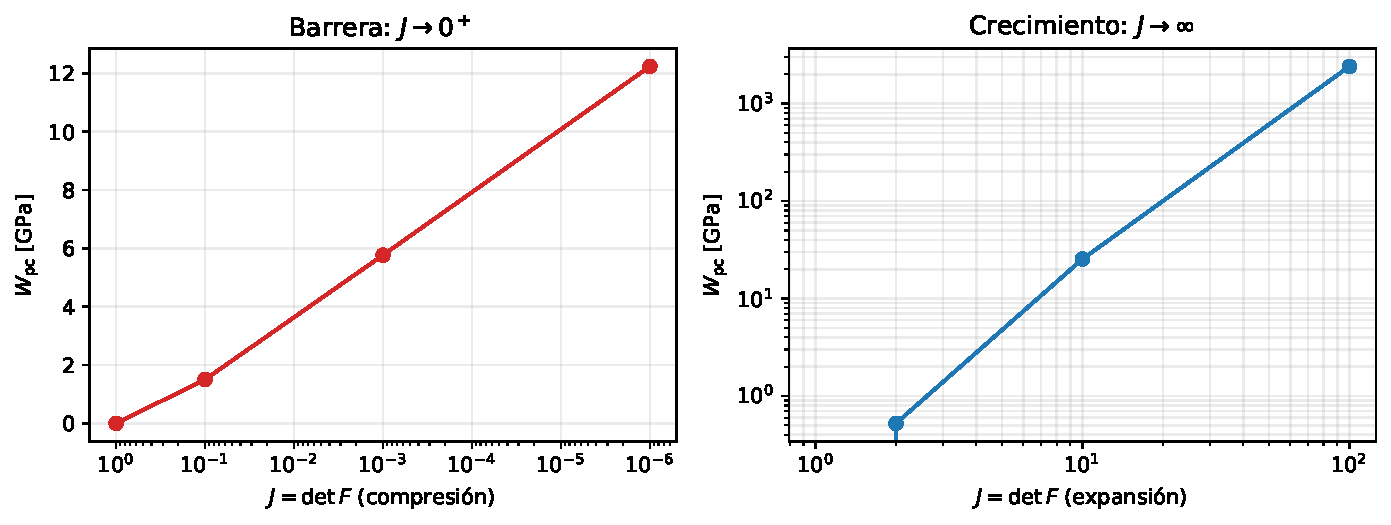
\includegraphics[width=0.92\linewidth]{polyconvex_d4_barrier.pdf}
 \caption{Auditoría volumétrica de \PConvPANN{} a lo largo de
\(\F=\operatorname{diag}(J,1)\). La energía diverge al colapsar el volumen
y crece sin cota al expandirse.}
 \label{fig:pc-barrier}
\end{figure}

\section{ICKAN: control directo y extensión policonvexa de menores}

Los ensayos ICKAN históricos no se mezclan con los resultados anteriores: el
mejor archivo heredado entrenaba y evaluaba sólo la trayectoria 3, con otra
medida de tensión. Ese experimento de reproducción dio \(6.27\%\) de error
global de tensión para ICKAN frente a \(1.64\%\) para ICNN, pero no responde a
la pregunta actual de generalización Stage--1/Stage--10. Por ello se hicieron
dos reentrenamientos desde cero con los \(109\,460\) estados Stage--1 y la
misma pérdida de energía y tensión de la ecuación~\eqref{eq:loss}.

\subsection{ICKAN directa: control de la representación spline}

La primera red conserva la entrada normalizada
\(\evec=[E_{xx},E_{yy},\gamma_{xy}]^T\). Una ICKAN escalar
\(3,8,1\), con splines cúbicos y malla fija de 15 intervalos, se promedia
sobre \(\Dfour\):
\[
 H_{\theta,\Dfour}^{\mathrm{dir}}(\evec)
 =\frac14\sum_{g\in\Dfour}K_\theta(g\evec),
 \qquad
 W_{\mathrm{dir}}=H_{\theta,\Dfour}^{\mathrm{dir}}(\evec)
 -H_{\theta,\Dfour}^{\mathrm{dir}}(\bm0)
 -\left.\frac{\partial H_{\theta,\Dfour}^{\mathrm{dir}}}{\partial\evec}
 \right|_{\bm0}\!\cdot\evec.
 \label{eq:ickan-direct}
\]
La última corrección garantiza referencia sin tensión y conserva convexidad
en \(\E\), pues sólo resta una función afín. No prueba policonvexidad: las
variables de entrada siguen siendo componentes de \(\E\), no los menores de
\(\F\). Su función es por tanto un control honesto: separa el efecto de usar
splines KAN del efecto de cambiar la estructura constitutiva.

\subsection{\texorpdfstring{\PConvICKAN{}}{PConv-ICKAN}: qué se restringe}

La segunda red usa las cuatro direcciones axiales y diagonales
\(\mathcal A_4\). Construye las ocho medidas de la
ecuación~\eqref{eq:directional_minors}, junto con \(J\) y \(J^2\), y sólo
aplica una normalización afín positiva, por ejemplo
\(\widehat q=(q-1)/s\) con \(s>0\). Esa normalización no altera convexidad
ni monotonía en la variable física \(q\).

Cada arista spline de ICKAN se escribe
\[
 \phi(x)=\sum_i N_{i,3}(x)c_i^\star,
 \qquad
 c_i^\star=c_1+\sum_{j\le i}\sum_{k\le j}\operatorname{ReLU}(\rho_k).
 \label{eq:ickan-spline}
\]
Así, los incrementos primero y segundo de los coeficientes son no negativos;
para un B-spline cúbico esto da \(\phi'(x)\ge0\) y
\(\phi''(x)\ge0\). En la implementación se usa además
\texttt{base\_fun=zero}, escalas spline positivas y sin rama simbólica. Las
sumas y composiciones de estas aristas siguen siendo convexas y no decrecientes
en cada entrada. No es una afirmación empírica sobre el Hessiano: es la
restricción estructural de la ICKAN \cite{thakolkaran2025}.

Por ello, si \(K_\theta\) denota dicha ICKAN, la energía usada es
\[
 H_{\theta,\Dfour}^{\mathrm{IK}}(\E)
 =\frac14\sum_{g\in\Dfour}K_\theta\!\left(
 \{\widehat q^F_{\bm a}(g\E),\widehat q^H_{\bm a}(g\E)\}_{\bm a\in\mathcal A_4},
 \widehat J(g\E),\widehat{J^2}(g\E)\right),
\]
\[
 \boxed{
 W_{\mathrm{IK}}(\E)=H_{\theta,\Dfour}^{\mathrm{IK}}(\E)
 -H_{\theta,\Dfour}^{\mathrm{IK}}(\bm0)
 -r\log J+\frac{\beta}{2}(J-1)^2,\qquad \beta>0.}
 \label{eq:pconv-ickan-energy}
\]
con \(r\) calculado mediante la ecuación~\eqref{eq:pc_reference_pressure}.
Por el mismo argumento de composición de la sección anterior,
\(W_{\mathrm{IK}}=G(\F,\operatorname{cof}\F,J)\) con \(G\) convexa. Por
tanto \PConvICKAN{} es objetiva, \(\Dfour\)-simétrica, energía--tensión
consistente, policonvexa y tiene barrera volumétrica. No se emplea la
corrección afín de la ecuación~\eqref{eq:ickan-direct} en esta variante, pues
destruiría esta prueba.

El checkpoint final tiene \(r=0.24145\) y \(\beta=0.005219\), ambos en
unidades normalizadas y positivos. La energía evaluada en
\(\F=\operatorname{diag}(J,1)\) crece de \(1.006\)~GPa en \(J=0.1\) a
\(3.377\)~GPa en \(J=10^{-3}\), y alcanza \(2491.9\)~GPa en \(J=100\).
En 32 caminos aleatorios de rango uno, la menor segunda derivada fue
\(0.437\)~GPa. Los residuos numéricos de referencia \(31.8\)~Pa y de energía
\(\Dfour\) \(254.6\)~Pa son redondeo de aritmética \texttt{float32} frente a
una escala de GPa.

\begin{figure}[ht]
 \centering
 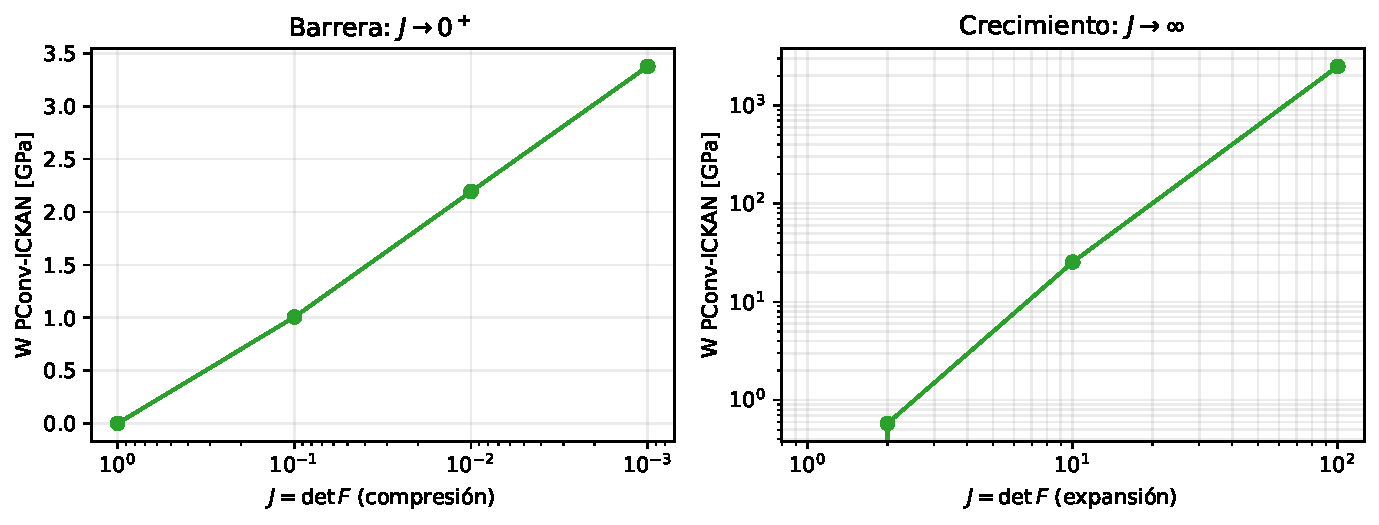
\includegraphics[width=0.92\linewidth]{ickan_d4_barrier.pdf}
 \caption{Auditoría volumétrica de \PConvICKAN{} a lo largo de
\(\F=\operatorname{diag}(J,1)\). La barrera y el crecimiento proceden de
la forma analítica de la ecuación~\eqref{eq:pconv-ickan-energy}.}
 \label{fig:ickan-barrier}
\end{figure}

\section{Evaluación final en Stage--10}

Después de la selección, la \PANN{} se reentrenó con las diez trayectorias
Stage--1 y se evaluó una única vez en Stage--10. La Tabla~\ref{tab:stage10}
compara los errores con la energía y tensión conjugada directas del \FOM.

\begin{table}[ht]
\centering
\small
\caption{Errores relativos \(L^2\) en la trayectoria Stage--10 frente al
\FOM{} directo. Cada PANN corresponde a una sola semilla.}
\label{tab:stage10}
\begin{tabular}{lrrrrr}
\toprule
Modelo & \(\W\) & \(\Svec\) global & \(S_{xx}\) & \(S_{yy}\) & \(S_{xy}\)\\
\midrule
\HPROM{} & \(0.000165\%\) & \(0.118\%\) & \(0.109\%\) & \(0.117\%\) & \(13.338\%\)\\
\PANN{} & \(\mathbf{0.0522\%}\) & \(\mathbf{0.1689\%}\) &
\(\mathbf{0.1650\%}\) & \(0.1729\%\) & \(\mathbf{0.7852\%}\)\\
\ICNN{} & \(1.589\%\) & \(3.632\%\) & \(4.103\%\) & \(3.075\%\) & \(38.961\%\)\\
\PConvPANN{} & \(10.751\%\) & \(11.225\%\) & \(10.275\%\) & \(12.117\%\) & \(36.838\%\)\\
\ICKAN{} directa & \(23.008\%\) & \(23.381\%\) & \(22.180\%\) & \(24.543\%\) & \(70.950\%\)\\
\PConvICKAN{} & \(2.106\%\) & \(2.635\%\) & \(2.203\%\) & \(3.012\%\) & \(9.544\%\)\\
\bottomrule
\end{tabular}
\end{table}

\begin{figure}[ht]
 \centering
 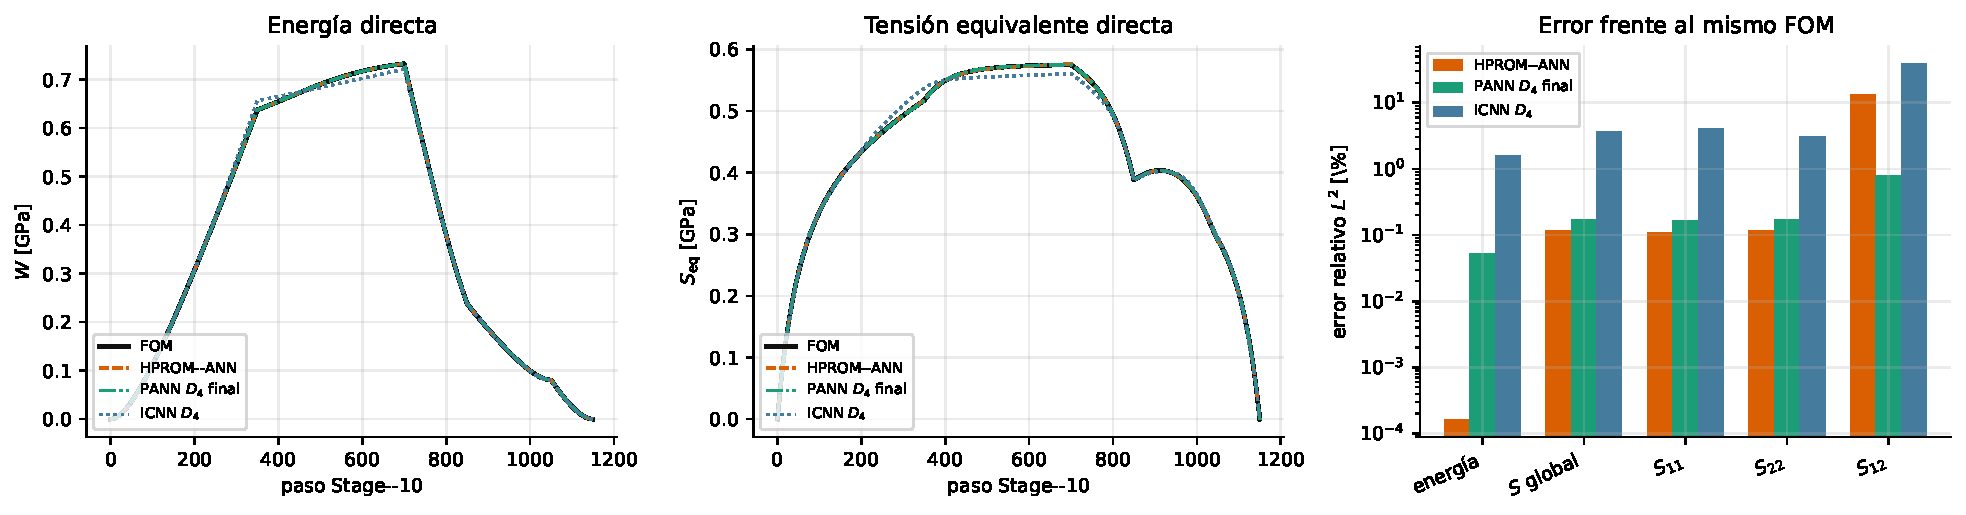
\includegraphics[width=0.92\linewidth]{stage10_final_comparison.pdf}
 \caption{Historias Stage--10 comparadas con la energía y tensión conjugada
directas del \FOM. La \PANN{} corresponde al modelo seleccionado con una sola
semilla.}
 \label{fig:stage10}
\end{figure}

La \HPROM{} conserva una ventaja clara en energía y en la norma global de
tensión. La \PANN{} es, sin embargo, muy superior a la \ICNN{} y aproxima la
componente de cizalla \(S_{xy}\) con un error de \(0.7852\%\), frente a
\(13.338\%\) de la \HPROM{} en esta comparación concreta.

La comparación anterior requiere una precaución de medida. Los ficheros
históricos de \HPROM{} y D--HPROM--ANN guardan una tensión promediada que no
coincide necesariamente con \(\partial\W^M/\partial\E\) a deformación finita.
Para la Tabla~\ref{tab:stage10}, la respuesta de \HPROM{} se reconstruyó en la
misma medida energía--tensión conjugada que usa la \PANN{}. No se deben mezclar
sin indicarlo los errores obtenidos frente a la tensión histórica con los
errores frente a la tensión energética directa.

La \PConvPANN{} se evalúa contra exactamente los mismos estados directos del
\FOM. Sus errores Stage--10, \(10.751\%\) en energía y \(11.225\%\) en
tensión global, son muy superiores a los de la \PANN{} libre. La
policonvexidad y la barrera no son gratis para esta clase de funciones y este
conjunto de datos. La Figura~\ref{fig:pc-stage10} permite localizar esa
diferencia: la respuesta sigue la forma macroscópica de la trayectoria, pero
subestima de manera sistemática una parte de la energía y las tensiones
normales. En particular, este modelo debe comunicarse como un \emph{baseline}
constitutivo garantizado, no como el reemplazo preciso de HPROM--ANN.

La \ICKAN{} directa confirma que cambiar una MLP por una red spline no basta:
su \(23.008\%\) de error energético y \(23.381\%\) de error de tensión son
los peores de la tabla. En cambio, el cambio constitutivo a menores
direccionales y la corrección volumétrica permiten a \PConvICKAN{} bajar a
\(2.106\%\) en energía y \(2.635\%\) en tensión. Es una mejora sustancial
respecto a \PConvPANN{} y también reduce la tensión global frente a \ICNN{};
sin embargo, su cizalla \(S_{xy}\) permanece en \(9.544\%\) y no compite con
la PANN libre. La conclusión no es ``KAN mejor que MLP'' en abstracto: para
este RVE, la ganancia viene de combinar la KAN monótona-convexa con los
menores adecuados y la barrera, pero la clase garantizada sigue siendo más
restrictiva que la aproximación libre.

\begin{figure}[ht]
 \centering
 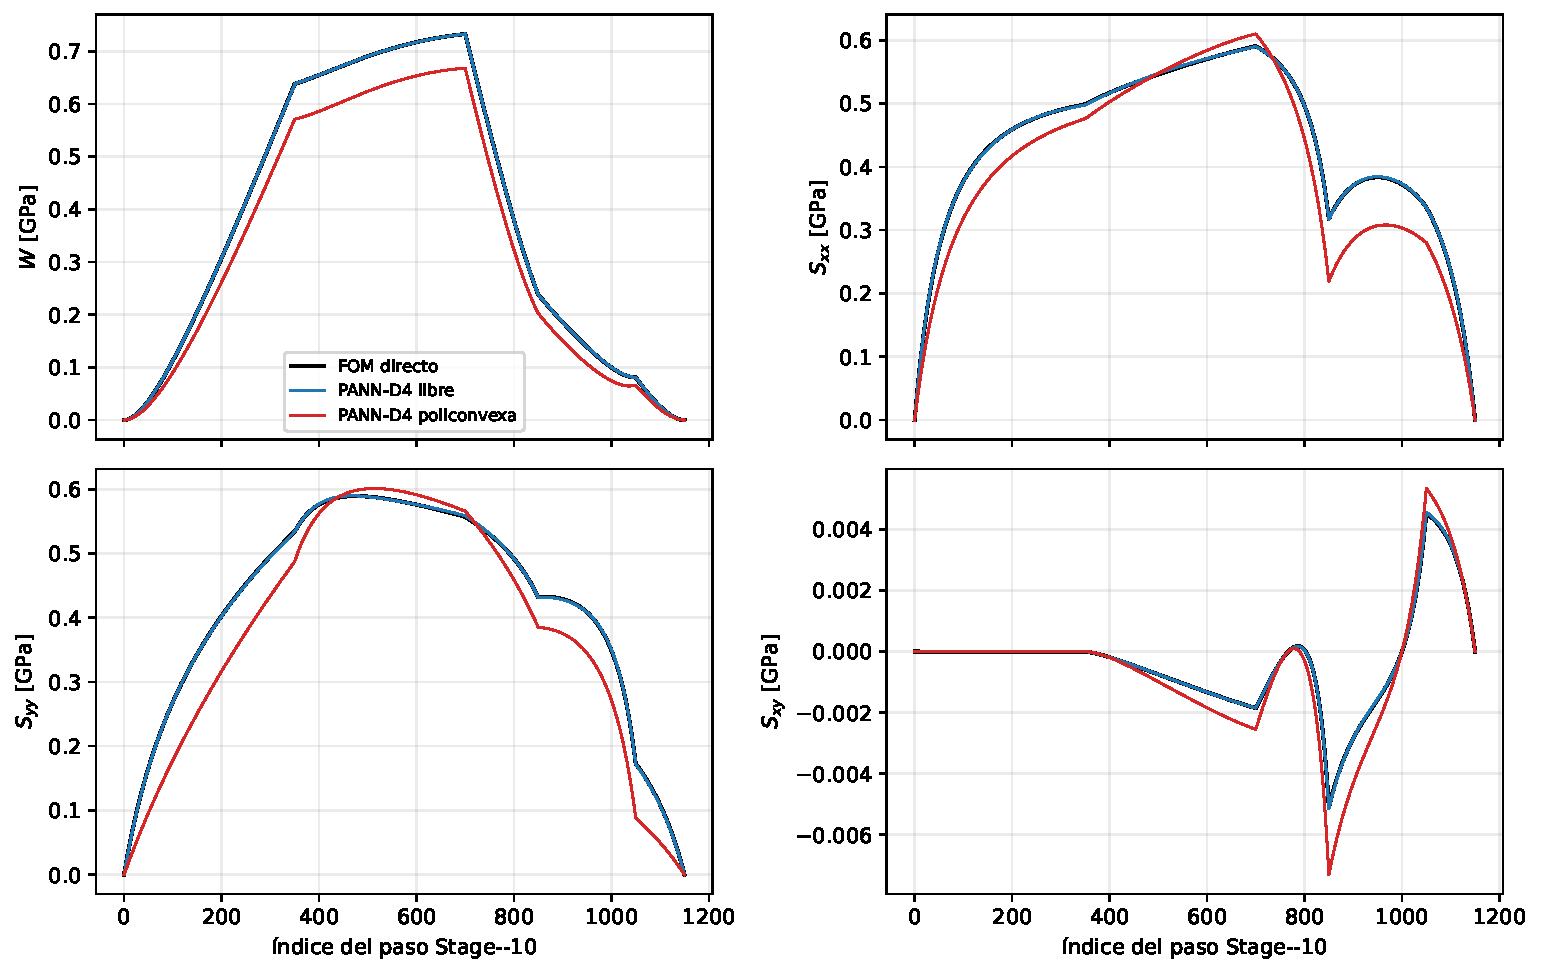
\includegraphics[width=0.94\linewidth]{polyconvex_d4_stage10_comparison.pdf}
 \caption{Stage--10: comparación directa del \FOM{}, la \PANN{} libre y la
\PConvPANN{}. La restricción policonvexa conserva estructura física global,
pero en la clase explorada reduce la fidelidad dentro del dominio de interés.}
\label{fig:pc-stage10}
\end{figure}

\begin{figure}[ht]
 \centering
 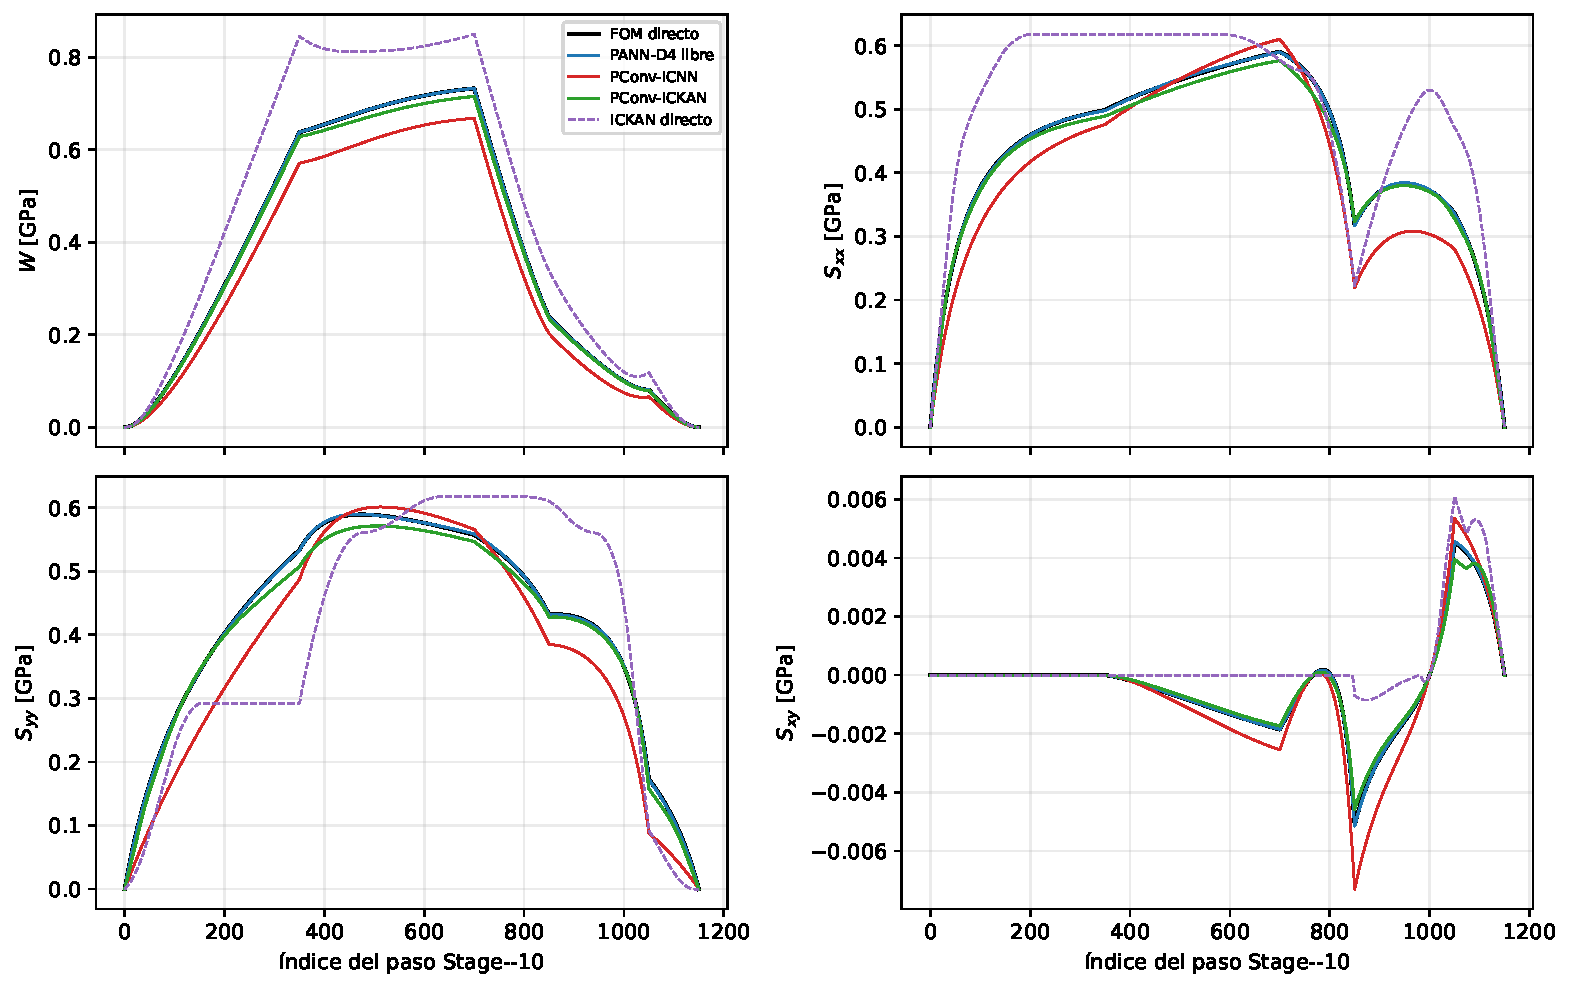
\includegraphics[width=0.96\linewidth]{ickan_d4_stage10_comparison.pdf}
 \caption{Stage--10 en la misma medida energética: \PANN{} libre,
\PConvPANN{}, \PConvICKAN{} e \ICKAN{} directa. La ICKAN directa se muestra
para documentar el control negativo; la \PConvICKAN{} reproduce mejor las
ramas normales que la PConv--ICNN, pero conserva error de cizalla apreciable.}
 \label{fig:ickan-stage10}
\end{figure}

\subsection{Reentrenamiento de verificación de la implementación compacta}

Como comprobación independiente, se reentrenó desde cero la \PANN{} con el
código compacto que promedia sólo las cuatro acciones distintas de
\(\Dfour\). Este promedio es matemáticamente idéntico al promedio sobre las
ocho matrices del grupo, donde cada acción tensorial aparece dos veces. Se
mantuvieron la arquitectura, la pérdida de la ecuación~\eqref{eq:loss}, los
\(109\,460\) estados Stage--1, la semilla \(20260731\), \(300\) épocas y el
tamaño de lote \(2\,048\). El mejor estado Stage--1 se obtuvo en la época 290,
con errores de entrenamiento de \(0.0317\%\) en energía y \(0.2033\%\) en
tensión global.

\begin{table}[ht]
\centering
\caption{Comprobación de reproducibilidad en Stage--10. La réplica no se usa
para seleccionar el modelo: Stage--10 permanece como test final.}
\label{tab:retraining}
\begin{tabular}{lccccc}
\toprule
Entrenamiento & \(\W\) & \(\Svec\) global & \(S_{xx}\) & \(S_{yy}\) & \(S_{xy}\)\\
\midrule
Checkpoint distribuido & \(0.0522\%\) & \(0.1689\%\) & \(0.1650\%\) &
\(0.1729\%\) & \(0.7852\%\)\\
Réplica compacta desde cero & \(0.0576\%\) & \(0.1747\%\) & \(0.1764\%\) &
\(0.1730\%\) & \(0.8153\%\)\\
\bottomrule
\end{tabular}
\end{table}

La concordancia confirma que la implementación de cuatro acciones reproduce
la respuesta del modelo seleccionado. La pequeña variación se atribuye a la
ruta numérica del entrenamiento en GPU, no a un cambio de formulación. No se
reemplaza el checkpoint distribuido usando el test Stage--10, ya que hacerlo
convertiría el test en un criterio de selección.

\section{Conclusiones y límites}

El trabajo ha establecido una PANN de energía para el RVE considerado con una
formulación que es coherente con su cinemática y con su simetría efectiva. La
\PANN{} libre seleccionada:
\begin{itemize}
\item recibe \([E_{xx},E_{yy},\gamma_{xy}]\), por lo que es objetiva;
\item impone exactamente la simetría material cuadrada \(\Dfour\), que fue
verificada en el \FOM{} y distinguida de isotropía completa;
\item impone exactamente energía y tensión nulas en referencia;
\item predice tensión como derivada de una única energía;
\item se seleccionó sin usar Stage--10 y alcanzó buena precisión en ese
ensayo final no visto.
\end{itemize}

Para explorar las garantías que esa arquitectura no posee, se construyó la
\PConvPANN{}. Esta segunda arquitectura sí es objetiva, \(\Dfour\)-simétrica,
normalizada, energía--tensión consistente, policonvexa en \(\F\), de rango
uno convexa y coerciva ante \(J\to0^+\) y \(J\to\infty\). Sin embargo, no
garantiza convexidad en \(\E\), ni reproduce Stage--10 con una precisión
competitiva frente a \PANN{} o HPROM--ANN. La conclusión racional actual es
por tanto doble: \PANN{} es el surrogate preciso para la comparación con
HPROM--ANN dentro del dominio de datos; \PConvPANN{} es una demostración
funcional de que las garantías globales son posibles para la simetría \(\Dfour\),
pero necesita una clase policonvexa más expresiva antes de ser candidato a
reemplazo de alta fidelidad.

La exploración ICKAN aclara dónde está esa expresividad. La \ICKAN{} directa
es un control negativo y queda descartada como surrogate predictivo. La
\PConvICKAN{} conserva las mismas garantías globales de \PConvPANN{} pero
mejora el test a \(2.106\%\) de energía y \(2.635\%\) de tensión global.
Es, por tanto, el mejor baseline policonvexo actual de este directorio y una
contribución metodológica defendible: prueba que una KAN adecuadamente
restringida puede combinar simetría \(\Dfour\), integrabilidad,
policonvexidad y una precisión moderada. No debe presentarse como sustituto
de HPROM--ANN o de la PANN libre, pues su cizalla y sus errores globales siguen
un orden de magnitud por encima.

\section*{Trazabilidad computacional}

El directorio \texttt{PANN\_D4} contiene el checkpoint seleccionado, los datos
compactos Stage--1/Stage--10, la arquitectura
\texttt{pann\_d4\_model.py}. El entrenamiento final se ejecuta con
\texttt{train\_pann\_d4.py} y la evaluación con
\texttt{evaluate\_pann\_d4.py}. La evaluación del checkpoint distribuido
reproduce \(0.0522\%\) de error en energía, \(0.1689\%\) en tensión global y
\(0.7852\%\) en cizalla en Stage--10.

La extensión garantizada se reproduce con:
\begin{itemize}
\item \texttt{polyconvex\_d4\_model.py}: arquitectura y certificado;
\item \texttt{train\_polyconvex\_d4.py}: ajuste con Stage--1;
\item \texttt{evaluate\_polyconvex\_d4.py}: Stage--10 y auditorías;
\item \texttt{make\_polyconvex\_d4\_figures.py}: figuras del informe.
\end{itemize}
El checkpoint correspondiente es
\texttt{PANN\_D4\_polyconvex\_best.pt}. Estos scripts entrenan sólo con
Stage--1; el evaluador es el único que abre Stage--10 para este candidato.

Los ensayos ICKAN se reproducen con:
\begin{itemize}
\item \texttt{ickan\_d4\_model.py}: ICKAN directa y \PConvICKAN{};
\item \texttt{train\_ickan\_d4.py}: entrenamiento Stage--1 desde cero;
\item \texttt{evaluate\_ickan\_d4.py}: evaluación Stage--10 y auditorías;
\item \texttt{make\_ickan\_d4\_figures.py}: figuras comparativas.
\end{itemize}
Los checkpoints \texttt{ICKAN\_D4\_direct\_best.pt} y
\texttt{ICKAN\_D4\_minor\_features\_best.pt} se seleccionan con métricas
Stage--1; sus evaluaciones Stage--10 se guardan por separado.

\begin{thebibliography}{9}
\footnotesize
\bibitem{aguila2026}
J.~Águila Martínez. \emph{Exploring the Use of Machine Learning Techniques in
Solid Mechanics Applications: A Study of Physics Enforcement Strategies Using
Synthetic Data}. Trabajo de Fin de Grado, UPC, 2026. Véanse especialmente los
apartados 3.5 y 4.5.

\bibitem{amos2017}
B.~Amos, L.~Xu y J.~Z.~Kolter. Input convex neural networks.
\emph{Proceedings of the 34th International Conference on Machine Learning},
2017.

\bibitem{gurtin2010}
M.~E.~Gurtin, E.~Fried y L.~Anand. \emph{The Mechanics and Thermodynamics of
Continua}. Cambridge University Press, 2010. Véase el Capítulo 50,
Material Symmetry.

\bibitem{nye1985}
J.~F.~Nye. \emph{Physical Properties of Crystals: Their Representation by
Tensors and Matrices}. Clarendon Press, Oxford, 1985.

\bibitem{ball1977}
J.~M.~Ball. Convexity conditions and existence theorems in nonlinear
elasticity. \emph{Archive for Rational Mechanics and Analysis},
63(4):337--403, 1977.

\bibitem{linka2023}
K.~Linka and E.~Kuhl. A new family of Constitutive Artificial Neural Networks
towards automated model discovery. \emph{Computer Methods in Applied Mechanics
and Engineering}, 403:115731, 2023.

\bibitem{thakolkaran2025}
P.~Thakolkaran, Y.~Guo, S.~Saini, M.~Peirlinck, B.~Alheit and S.~Kumar.
Can KAN CANs? Input-convex Kolmogorov--Arnold networks as hyperelastic
constitutive artificial neural networks. \emph{Computer Methods in Applied
Mechanics and Engineering}, 2025. doi:10.1016/j.cma.2025.118089.
\end{thebibliography}

\end{document}
